\documentclass[a4paper, 11pt]{article}

\usepackage[utf8]{inputenc}
\usepackage{babel}
\usepackage{amsmath}
\usepackage{a4wide}
\usepackage{relsize}
\usepackage{hyperref}
\usepackage[capitalise, noabbrev]{cleveref}
\usepackage{nameref}
\usepackage{indentfirst}
\usepackage{graphicx}
\usepackage{float}
\usepackage[normalem]{ulem}
\usepackage[bottom]{footmisc}
\usepackage{setspace}
\usepackage{tikz-cd}

\onehalfspacing

\title{Security and Applications in Trusted Hardware \\ [.8em] \smaller Portable Password Manager}
\author{João Silva \and Rui Fernandes \and Tiago Garcia}
\date{\today}

\renewcommand\labelitemi{--}
\renewcommand{\today}{\ifcase \month\or January\or February\or March\or %
April\or May\or June\or July\or August\or September\or October\or November\or %
December\fi, \number \year}

\hypersetup{
    pdftitle={Portable Password Manager},
    pdfborder={0 0 0}
}

\begin{document}

    \begin{titlepage}
        \begin{center}
            \begin{minipage}{.75\linewidth}
                \centering
                
\includegraphics[width=0.5\textwidth]{img/fcup}\par\vspace{1cm}
                \vspace{1.5cm}
                {\scshape\LARGE Faculty of Sciences of the University of Porto} \par
                \vspace{1cm}
                {\scshape\Large Master's Degree in Information Security} \par
                \vspace{1.5cm}
                \maketitle
            \end{minipage}
        \end{center}
        \vspace{2cm}
        \thispagestyle{empty}
        \pagebreak
    \end{titlepage}

    \pagenumbering{roman}

    \begin{abstract}
        This report describes the practical assignment of the Security and Applications in Trusted Hardware
        course of the Master's Degree in Information Security at the Faculty of Sciences of the University
        of Porto.

        In this report, we briefly describe the application we developed and discuss the decisions we made.
    \end{abstract}

    \pagebreak

    \tableofcontents
    \listoffigures

    \pagebreak

    \pagenumbering{arabic}


    \section{Introduction}\label{sec:introduction}

    Smart cards have become more affordable as their computing capability and storage capacity have increased,
    opening doors to a wider range of security measures, making them perfect candidates for authentication
    devices.

    Smart cards' security mechanisms, together with their multi-application operating systems, allow for
    a wide range of uses.
    They are, for example, frequently utilized in public transportation application, such as Andante
    ~\cite{Transpor0:online}.
    Other use cases include functionalities related to authentication and digital signature (\textit{e.g.} Chave Móvel
    Digital~\cite{AChaveMo50:online}).

    In this report, we explore the use of smart cards in privacy-sensitive applications, namely password
    managers, provide an overview of existing solutions and discuss why they may not be adequate in certain scenarios.
    Finally, we propose a solution consisting in a password manager using a smart card simulator.

    \vspace{1.5\baselineskip}

    \subsection*{Structure of the Report}

    The remainder of the report is structured as follows:

    \begin{itemize}
        \item \cref{sec:problem},~\textbf{\nameref{sec:problem}}, describes the problem of password
        re-usage across multiple services and addresses existing solution to this problem.
        \item \cref{sec:solution},~\textbf{\nameref{sec:solution}}, describes the architecture of our
        proposed solution to the problem of password re-usage across multiple services, and discusses some implementation
        details.
        \item \cref{sec:conclusion},~\textbf{\nameref{sec:conclusion}}, concludes the report and
        suggests areas of future improvement.
    \end{itemize}

    \pagebreak


    \section{Problem} \label{sec:problem}

    Current authentication schemes are based on something the user has (\textit{e.g.} a smart card or a
    security token), something the user knows (\textit{e.g.} a password or a PIN), or their physical
    characteristics (\textit{e.g.} a fingerprint or iris pattern)~\cite{1246384}, being password-based
    authentication the most widely used.

    One problem with password-based authentication is that infrequently used passwords are easy to forget, and it is hard
    to remember secure passwords.
    In fact, to avoid memorizing numerous passwords, users tend to re-use the same password on different platforms
    ~\cite{florencio2006a}.
    As a result, discovering a user's password grants an attacker access to multiple of the user's systems.
    Some solutions address this issue by requiring users to remember only one password.

    \subsection{Existing Solutions} \label{subsec:solutions}

    In this section, we describe two different solutions to the problem of password re-use across
    multiple services, namely Single Sign On and Password Managers.

    \subsubsection{Single Sign On}

    User authentication can be delegated to an external service, known as Single Sign On (SSO).
    The purpose of such services is to authenticate users and securely communicate successful authentication to the services
    the user wants to use.
    This way, users only need to remember the password they use for the SSO service.
    Examples of SSO services include Shibboleth~\cite{10.1007/978-3-642-37282-7_14}.

    The main issue with this approach is their \uline{low portability} and their \uline{availability}, or lack thereof.
    For one thing, the service to which the user wants to authenticate must trust the SSO system.
    If this is not the case, the user still needs to remember a new password for the service.
    In other words, SSO systems only work with services that trust them.

    On the other hand, a service may not trust a SSO system due to the lack of availability guarantees.
    In other words, in case of a denial of service (DoS), the SSO may be disabled or
    rendered inaccessible, restricting user's ability to authenticate themselves.

    \subsubsection{Password Managers}

    Password managers are designed to store and provide access to a user's passwords.
    The user only needs to memorize a \textit{master password} and store his passwords in the password manager.
    Examples of password managers include Bitwarden~\cite{Bitwarde48:online} and KeePass~\cite{KeePassP1:online}.

    End-to-end encryption ensures that only the user has access to their master password and password vault -- it cannot
    be accessed by the service provider or intercepted by hackers.
    However, since no one else can access the user's data, it is crucial that they remember the master password.
    Moreover, in order to safely store the passwords, symmetrical ciphers (\textit{e.g.} AES) are used.
    These algorithms use either the master password, or a transformation of it such as its hash value,
    as a key to encrypt the stored data.
    However, other solutions exist.
    For example, by default, Firefox does not require a master password, using a default key to cipher passwords database.

    Finally, despite being more resistant to DoS attacks, password managers are still susceptible to brute-force attacks.

    \pagebreak


    \section{Proposed Solution} \label{sec:solution}

    \subsection{Security Requirements}\label{subsec:security-requirements}

    As any password manager, this eliminates the user need to remember multiple passwords.
    Thus, the following security requirements must be met:

    \begin{itemize}
        \item The password manager should be capable of generating complex, random passwords.
        \item Recovery of the master key should not be allowed.
        \item It shouldn't be possible to access passwords without the correct decryption key.
        \item If the smart card (which contains the decryption key) is lost, it should not be possible to recover data.
        This limits usability but makes the system more secure.
    \end{itemize}

    Unlike other existing solutions, we do not store the passwords in the card itself.
    Instead, it is only used as a means to perform encryption and decryption, and to generate random passwords.
    Smart cards are especially well suited for this type of application since they are extremely secure by design, and
    tampering leads in the destruction of the information stored therein.

    Finally, the use of smart cards in this application has the following benefits:

    \begin{itemize}
        \item \textbf{Applet isolation:} Different applets can safely coexist in the same card.
        Each applet is assigned to an execution context that controls access to the objects assigned to it.
        The boundary between one execution context and another is often called an \textit{applet
        firewall}~\cite{AnIntrod42:online}.
        \item \textbf{Cryptographic Operations:} The cryptographic key stored on the card is very well protected both
        physically and logically, and are therefore extremely hard to steal.
        In fact, the card contains security features that enable the protection of sensitive cryptographic data and
        provides a secure processing environment.
        Finally, it allows us to perform cryptographic operation without never revealing the key that was used.

    \end{itemize}

    \subsection{Assumptions}\label{subsec:assumptions}

    In this work, we make the following assumptions:

    \begin{itemize}
        \item The card is tamper-proof.
        Thus, it is not possible for an attacker to access the cryptographic key without previous authentication.
        \item Only the user knows the smart card access PIN. This means that if somebody authenticates
        with the user PIN, he is the expected user.
    \end{itemize}

    \subsection{Architecture}\label{subsec:architecture}

    The architecture of the proposed solution is illustrated in \cref{fig:arch}:

    \begin{figure}[H]
        \centering
        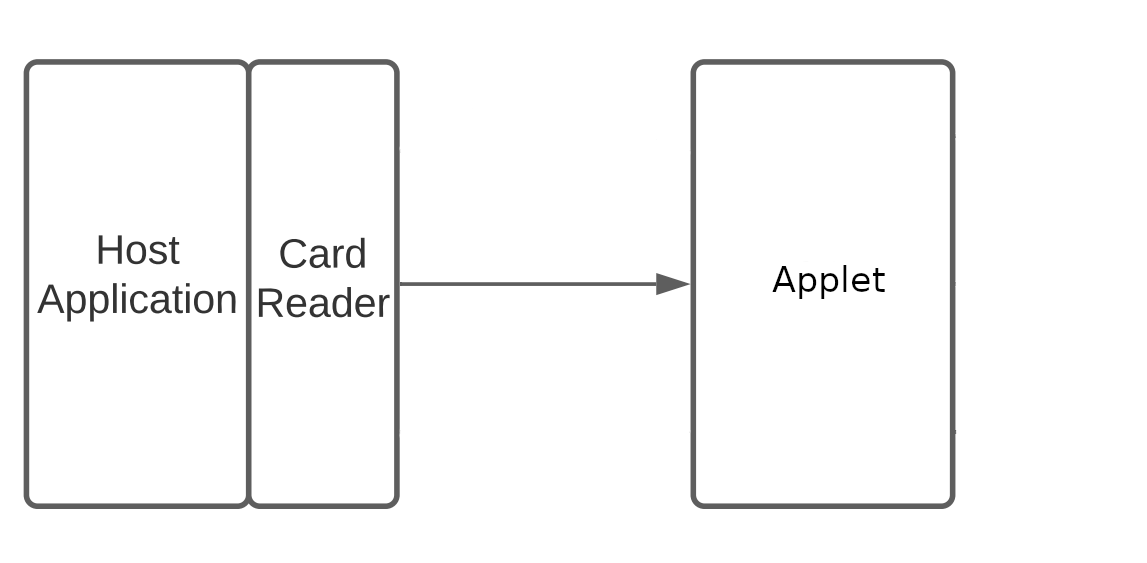
\includegraphics[width=.6\textwidth]{img/arch}
        \caption{System Architecture}
        \label{fig:arch}
    \end{figure}

    Here, a request-response protocol is used to communicate with the host application, in which application protocol data
    units (APDUs) are exchanged.

    In total, there are three entities:

    \begin{itemize}
        \item \textbf{Host application:} Responsible for storing the encrypted passwords (generated by the Java Card) in
        a SQL database.
        \item \textbf{Card Acceptance Device (CAD):} Responsible for making requests to the Java Card and
        forward the reply to the host application.
        \item \textbf{Java Card:} Responsible for authenticating the user, generating random passwords, as well as
        performing encryption and decryption operations.
    \end{itemize}

    Essentially, the card support two operations: \uline{generating} and \uline{retrieving} passwords, which will be
    addressed in more detail in the following sections.

    \subsubsection{Password Generation}

    To generate a password, 16 random bytes are generated, which are then encrypted using the AES master key.
    Then, the password is sent to the host application\footnote{The AES encrypted password is then encrypted once again
    using the CAD's public key.}, which is stored in a database, together with a description.

    This is illustrated in the following sequence diagram:

    \begin{figure}[H]
        \centering
        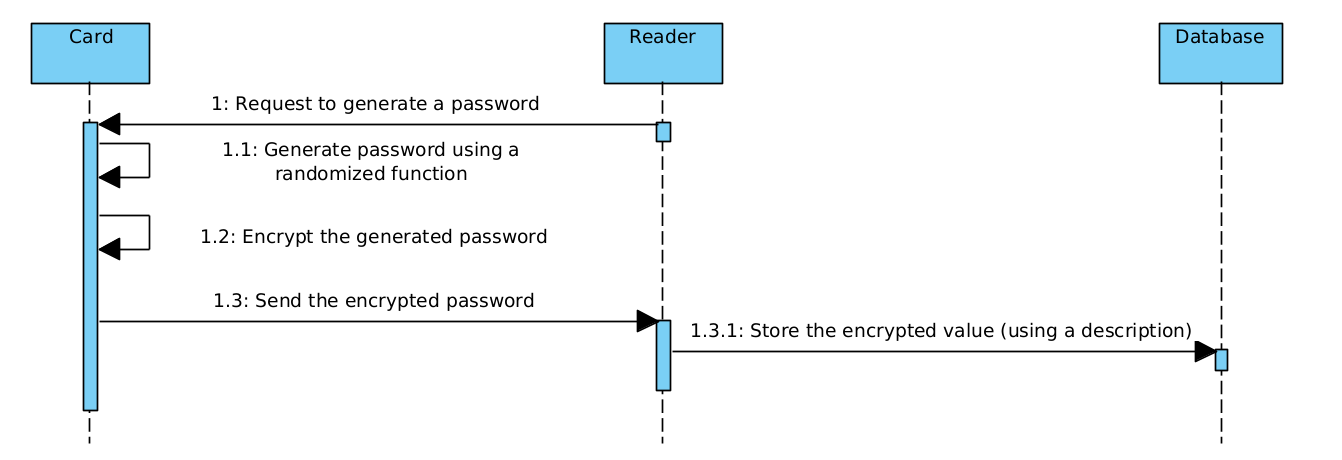
\includegraphics[width=\textwidth]{img/generation}
        \caption{Password Generation}
        \label{fig:generation}
    \end{figure}

    Here, it is worth noting that the password never leaves the smart card.
    This means that even if the whole database is compromised, the attack cannot decrypt the passwords because he does
    not have access to the key that was used to encrypt them, which is stored in the Java Card.

    \subsubsection{Password Retrieval}

    To retrieve a password, the encrypted password is first retrieved from the database based on the description provided
    by the user.
    The Java Card then decrypts this password using the AES master key stored therein, and returns it to the host
    application.
    Here, the password is not returned in plaintext -- before returning, the card encrypts the password with the CAD's
    public key.
    This way, an eavesdropper cannot intercept the password, and the received message is then decrypted with the CAD's
    private key and, finally, the password is shown to the user.

    This is illustrated in the following sequence diagram:

    \vspace{1.5\baselineskip}

    \begin{figure}[H]
        \centering
        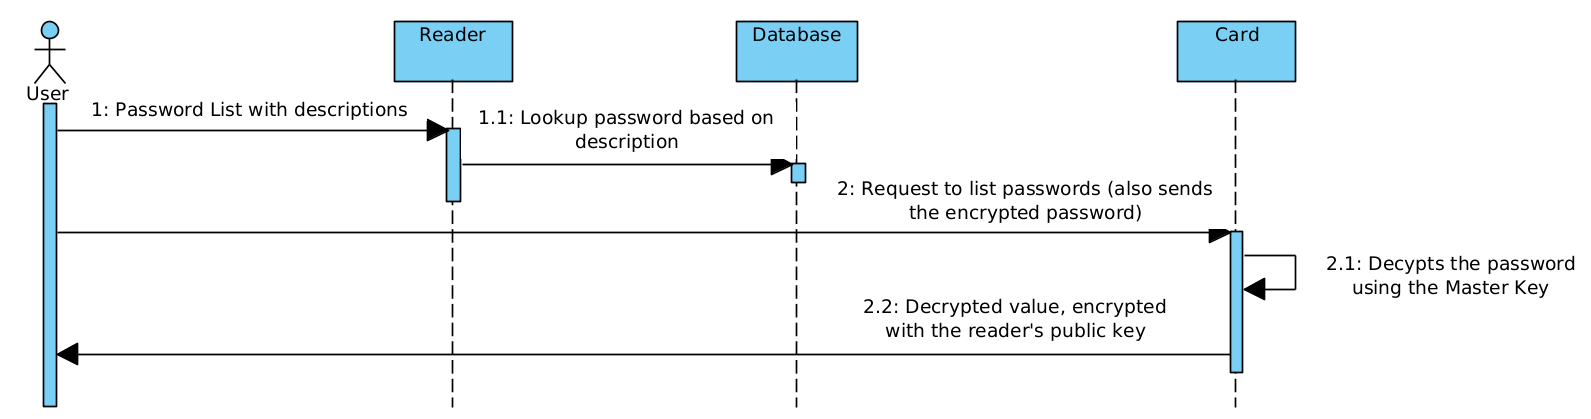
\includegraphics[width=\textwidth]{img/retrtieve}
        \caption{Password Retrieval}
        \label{fig:retrieve}
    \end{figure}

    \pagebreak

    \subsection{Attacks}\label{subsec:attacks}

    As mentioned in \cref{sec:conclusion}, due to time constraints, communication between the Java Card and the CAD is
    not encrypted.
    In an ideal scenario, this would be encrypted using a public key encryption scheme (\textit{e.g.} RSA or ECC), which
    would prevent eavesdropping in the sense that an attacker, even if capable of intercepting messages, would not be
    able to make sense of the data being transmitted.

    Under these circumstances, because communication is not being encrypted, the system is susceptible to \textit{replay
    attacks}, as illustrated in \cref{fig:replay-attack}.
    In this case, an eavesdropper could capture a message, say $msg_1$, drop it, modify it, and retransmit the resulting
    message, $msg_1'$, and the receiver would have no way of knowing that the message has been altered.

    \vspace{1.5\baselineskip}

    \begin{figure}[H]
        \centering
        \begin{tikzcd}
            Card                     &  &  &  & Eavesdropper                     &  &  &  & CAD \\
            {} \arrow[rrrr, "msg_1"] &  &  &  & {}                               &  &  &  &     \\
            &  &  &  & \text{Eavesdropper drops } msg_1 &  &  &  &     \\
            &  &  &  & {} \arrow[rrrr, "msg_{1}'"]      &  &  &  & {}
        \end{tikzcd}
        \caption{Replay attack}
        \label{fig:replay-attack}
    \end{figure}

    \vspace{1.5\baselineskip}

    However, as mentioned, it is quite straightforward to solve this problem -- it only requires encrypting communication.

    \pagebreak


    \section{Conclusion \& Future Work} \label{sec:conclusion}


    Due to some difficulties in setting up the development environment, we were not able to implement all the
    functionalities as initially planned.

    For one thing, communications between the Java card and the card acceptance device (CAD) are not encrypted.
    To do this, communication from the Java Card to the CAD would be encrypted with the CAD's public key, which would
    then be decrypted with its private key.
    On the other hand, communication from the CAD to the card would be encrypted with the card's public key, which would
    then be decrypted with the corresponding private key.
    To achieve this, it would be necessary to use public key encryption schemes such as RSA or ECC\@.

    Additionally, two more approaches could be optimized regarding the implementation of this work. Firstly, the current work is 
    generating a completely random password, meaning the bytes generated might not correspond to a classical 
    password (with only letters, numbers and special characters).
    Secondly, since this work relied only on the simulator, a few limitations were discovered, in particular 
    regarding the random bytes generated by this simulator. The first limitation was that the tool was incapable of 
    supporting the SECURE_RANDOM algorithm. The second limitation was that each time the card was booted, the same seed would be 
    inserted into the PSEUDO_RANDOM algorithm, which lead to the same passwords being generated every time the card was rebooted.

    To conclude, despite such difficulties, we still managed to achieve a functional implementation of a password
    manager with respect to the specification.
    This allowed us to have a better understanding of the specificities of developing an application that make use of
    smart cards.

    \pagebreak

    \bibliographystyle{IEEEtran}
    \bibliography{refs}
\end{document}
